\documentclass{article}

\usepackage{geometry}
\geometry{a4paper,margin=1in,}

\usepackage{hyperref}
\usepackage{graphicx}
\usepackage{float}

\title{COSC345 App Proposal}
\author{Name 1 (ID 1) Name 2 (ID 2) \\ Name 3 (ID 3) Louis Whitburn (2548261)}
\date{\today}

\begin{document}
	\maketitle
	
	We plan to build an Android app that allows the user to download / view course material from the COSC website \url{cs.otago.ac.nz}, and potentially, the MATH/STAT department website (\url{maths.otago.ac.nz})
	
	We intend to use Kotlin and target Android API level 28 (Android version 9, released August 6, 2018), however this target is very easy to change, as we don't expect to be using any very modern Android features. The app itself will work typically by guessing the correct page (e.g. \url{cs.otago.ac.nz/cosc345/lectures.php}) and enumerating PDFs, or by enumerating sub-pages of e.g. \url{cs.otago.ac.nz/cosc345}
	
	Main risk is the format changing. Consider the \url{cs.otago.ac.nz/cosc345/lectures.php} example, it is very possible that (intentionally or not) for some paper it might have another name. A real world example of this is \url{mark326@cs.otago.ac.nz} and \url{marks243@cs.otago.ac.nz}
	
	It will take ??? to build.
	
	\begin{figure}[h!]
		\centering
		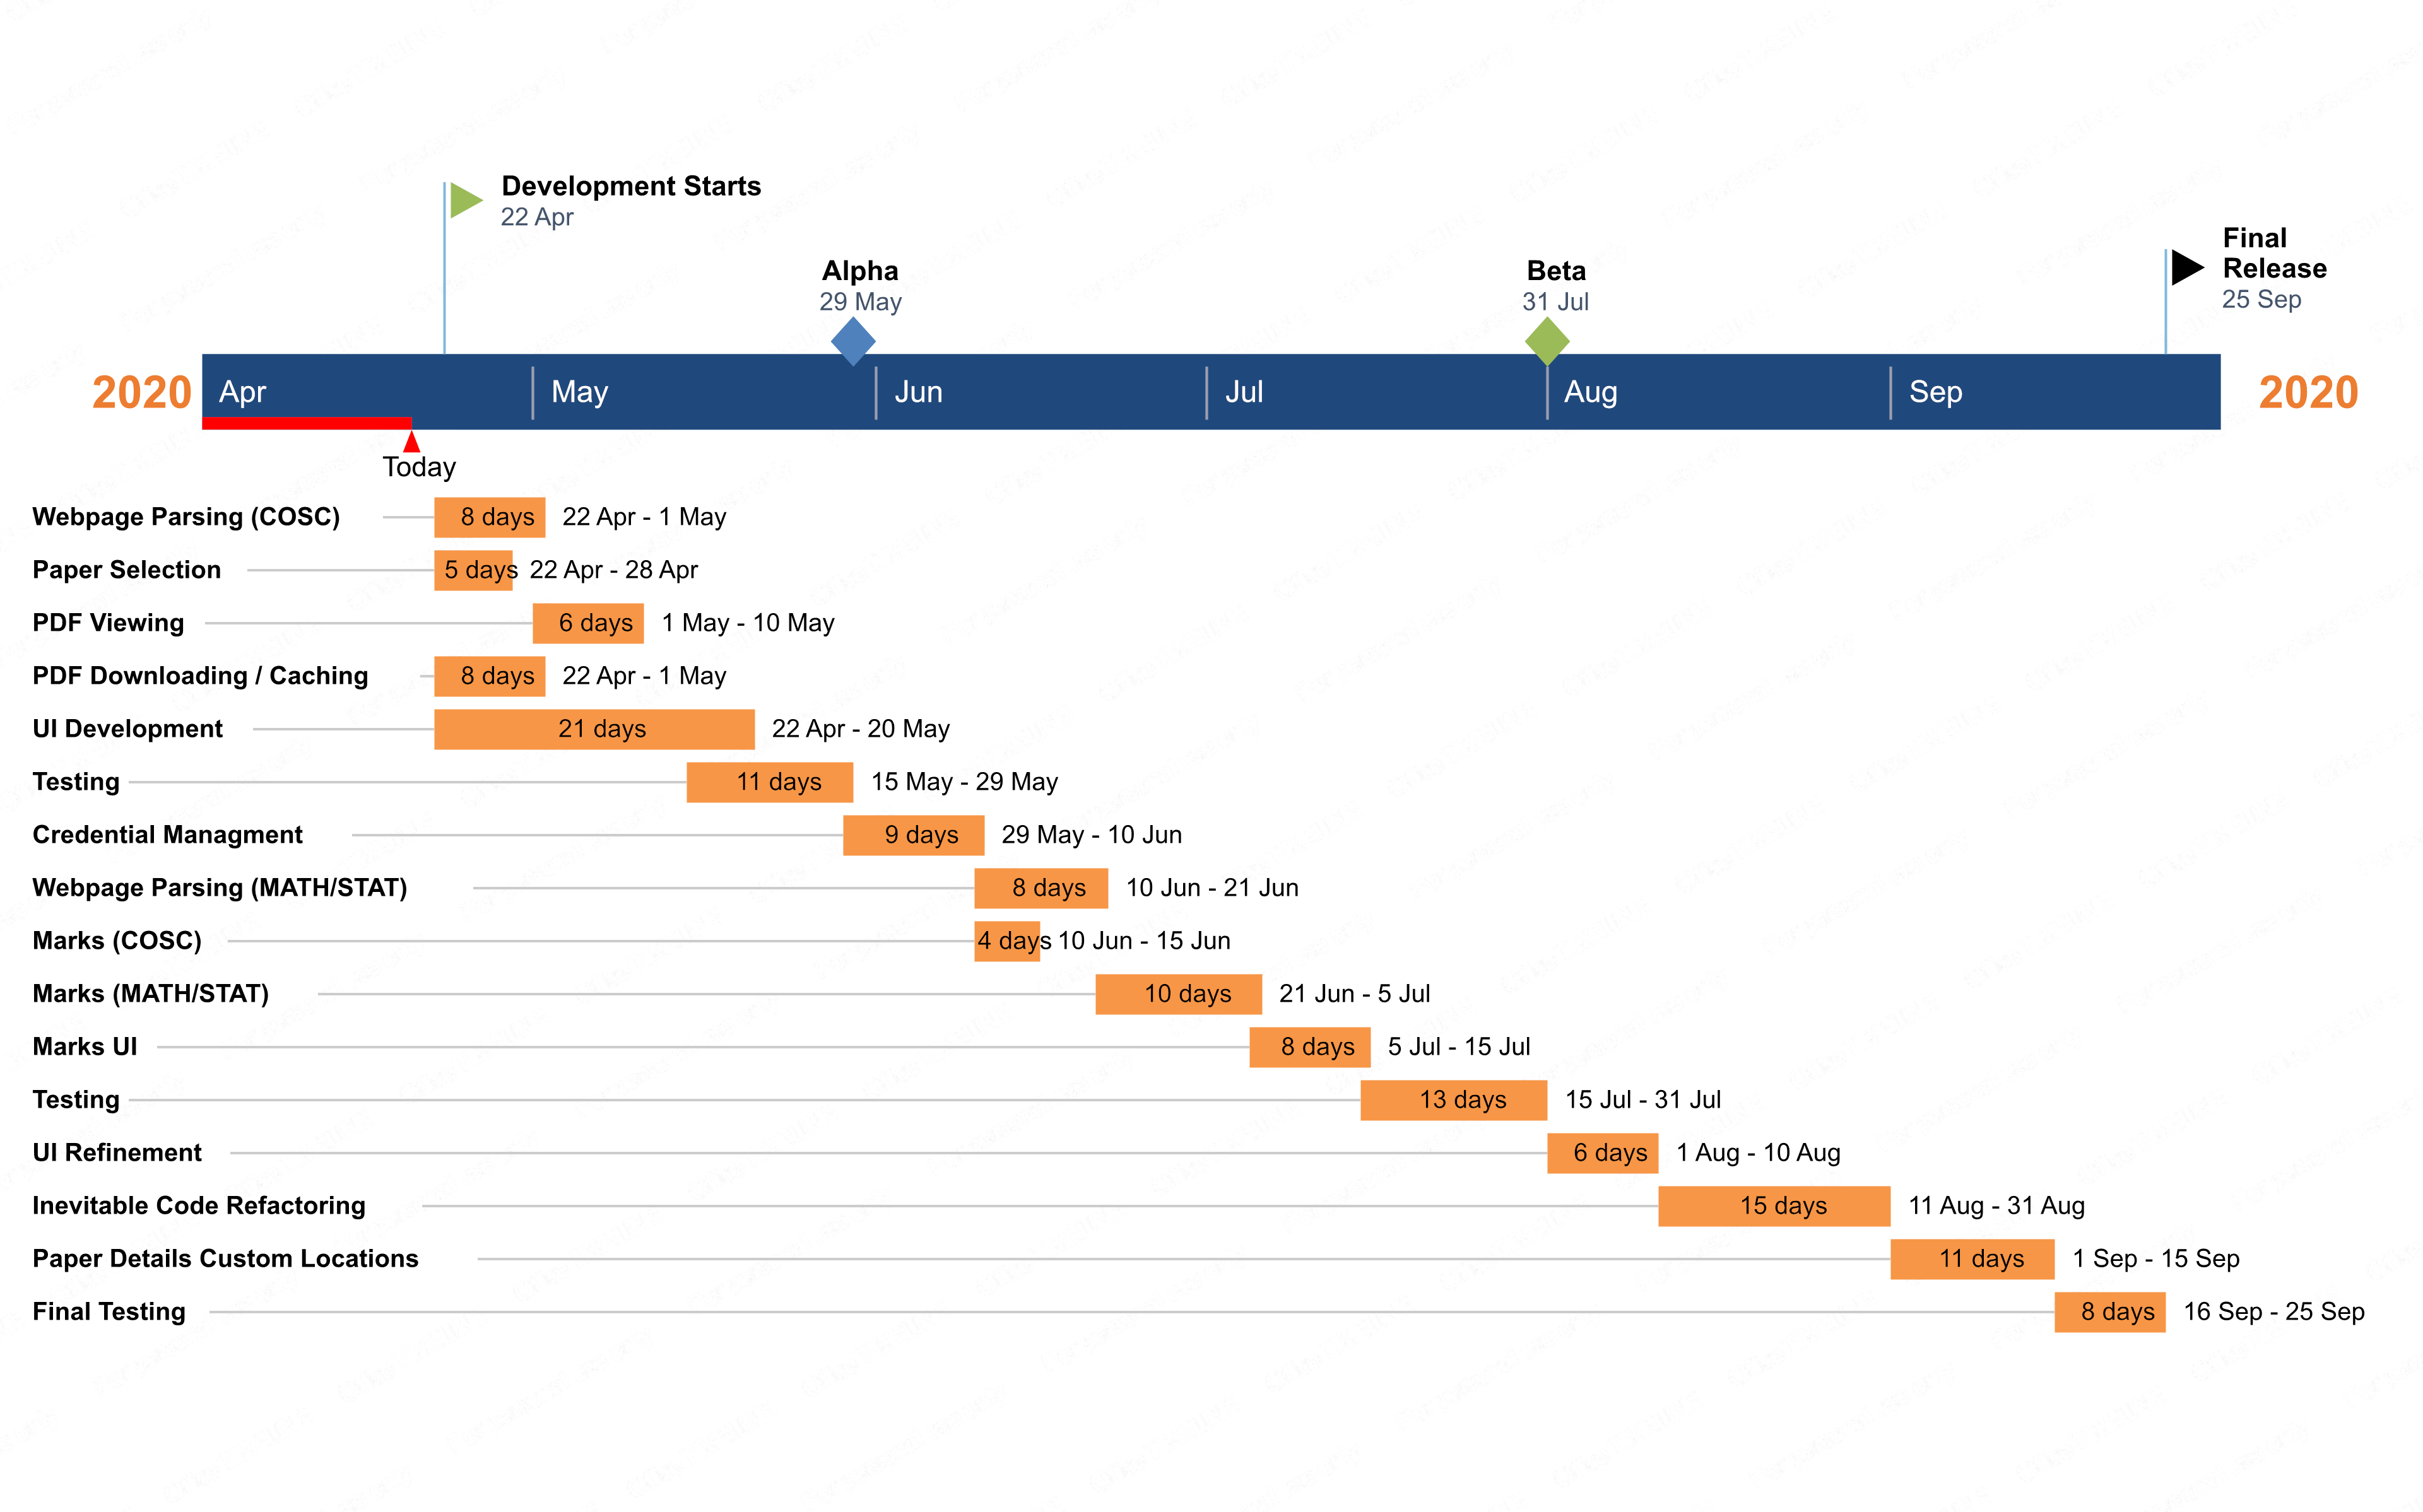
\includegraphics[width=\linewidth]{chart.png}
	\end{figure}
	
	Establishment has the \url{cs.otago.ac.nz} website, however navigating it on mobile is not a great experience.
	
	This will irritate the establishment since we will be creating a better version of what they already have - and will use the establishment's own gitlab server to do so. This will irritate people since the COSC department likes to do everything themselves, even if it occasionally breaks. In addition, having someone scrape your website and download a bunch of PDFs is possible irritating to some people.
\end{document}